\documentclass{article}

\setlength{\headsep}{0.75 in}
\setlength{\parindent}{0 in}
\setlength{\parskip}{0.1 in}

%=====================================================
% Add PACKAGES Here (You typically would not need to):
%=====================================================

\usepackage{xcolor}
\usepackage[margin=1in]{geometry} % Used for page margins, often replaces fullpage
\usepackage{amsmath,amsthm,amssymb} % amssymb added for common math symbols

\usepackage{enumitem} % For custom list environments

\usepackage{tcolorbox}
% \usepackage{fullpage} % Geometry handles this better
\usepackage[parfill]{parskip} % For paragraph spacing
\usepackage{hyperref}
\usepackage[nameinlink, capitalise]{cleveref} % For smart referencing

\usepackage{algorithm2e} % For algorithms
\usepackage{tikz} % For drawing diagrams
\usepackage{siunitx} % For units
\usepackage{graphicx}

\usetikzlibrary{arrows.meta, positioning}

\crefname{algocf}{Algorithm}{Algorithms}

\RestyleAlgo{ruled} % Style for algorithms

\definecolor{linkc}{rgb}{0.1, 0.5, 0.7}
\definecolor{citec}{rgb}{0.6, 0.3, 0.7}
\definecolor{urlc}{rgb}{0.5, 0.1, 0.2}
\hypersetup{
  colorlinks=true,
  linkcolor=linkc,
  citecolor=citec,
  urlcolor=urlc
}

\renewcommand{\d}{\,\mathrm{d}} % Differential d

%=====================================================
% Ignore This Part (But Do NOT Delete It:)
%=====================================================

\theoremstyle{definition}
\newtheorem{problem}{Problem}
\newtheorem*{fun}{Fun with Algorithms}
\newtheorem*{challenge}{Challenge Yourself}
\def\fline{\rule{0.75\linewidth}{0.5pt}}
\newcommand{\finishline}{
  \begin{center}\fline
\end{center}}
\newtheorem*{solution*}{Solution}
\newenvironment{solution}{
\begin{solution*}}{{\finishline}
\end{solution*}}
\newcommand{\grade}[1]{\hfill{\textbf{($\mathbf{#1}$ points)}}}
\newcommand{\thisdate}{\today}
\newcommand{\thissemester}{\textbf{Rutgers: Spring 2026}}
\newcommand{\thiscourse}{CS 344: Algorithms}
\newcommand{\thishomework}{Number}
\newcommand{\thisname}{Name}
\newcommand{\thisextension}{Yes/No}

\headheight 40pt
\headsep 10pt

\newcommand{\thisheading}{
  \noindent
  \begin{center}
    \framebox{
      \vbox{\vspace{2mm}
        \hbox to 6.28in { \textbf{\thiscourse \hfill \thissemester} }
        \vspace{4mm}
        \hbox to 6.28in { {\Large \hfill Homework \#\thishomework \hfill} }
        \vspace{2mm}
        \hbox to 6.28in { { \hfill \hfill} }
        \vspace{2mm}
        \hbox to 6.28in { \emph{Name(s): \thisname \hfill }}
      \vspace{2mm}}
    }
  \end{center}
  \bigskip
}

%=====================================================
% Some useful MACROS (you can define your own in the same exact way also)
%=====================================================

\newcommand{\ceil}[1]{{\left\lceil{#1}\right\rceil}}
\newcommand{\floor}[1]{{\left\lfloor{#1}\right\rfloor}}
\newcommand{\prob}[1]{\Pr\paren{#1}}
\newcommand{\expect}[1]{\Exp\bracket{#1}}
\newcommand{\var}[1]{\textnormal{Var}\bracket{#1}}
\newcommand{\set}[1]{\ensuremath{\left\{ #1 \right\}}}
\newcommand{\poly}{\mbox{\rm poly}}

%=====================================================
% Fill Out This Part With Your Own Information:
%=====================================================

\renewcommand{\thishomework}{3} %Homework number
\renewcommand{\thisname}{Iris Martinez} % Enter your name here

\begin{document}

\thisheading

\subsection*{Homework Policy}
\begin{itemize}
  \item You may consult all course materials (lecture notes, textbook, slides, etc.) while writing your solutions. No external resources are permitted.

  \item \textbf{All submissions should be typeset in LaTeX, handwritten solutions are not accepted}.

  \item Remember to always \textbf{prove the correctness} of your algorithms and \textbf{analyze their running time} (or any other efficiency measure asked in the question).

  \item Homework assignments are completed and submitted in fixed groups of 3 students. Only \textbf{one member of the group submits} the full solution on Canvas. The submission must include the names of all group members. The other two members do \textbf{not need to submit anything separately}.

  \item You may discuss the problems with any of your classmates, even those outside your group. However, \textbf{each group must write and submit their solutions independently}.

  \item Attempt the challenge problems only if you find them interesting.
\end{itemize}

\subsection*{Acknowledgment (to be reviewed and edited as needed)}
\begin{tcolorbox}[colframe=black,colback=white,arc=5mm]
  I, \textbf{Iris Martinez}, worked on this assignment individually.\textbf{I hereby affirm that all external assistance utilized in the preparation of this document has been properly acknowledged}.
\end{tcolorbox}

\finishline
\newpage

\newpage

\begin{problem}
  You are given an array of characters $S[1:n]$ such that each $S[i]$ is a small case letter from the English alphabet.
  You are also provided with a black-box algorithm $dict$ that given two indices $i,j \in [n]$, $dict(i,j)$ returns whether the sub-array $S[i:j]$ in array $S$ forms a valid word in English or not in $O(1)$ time. (Note that this algorithm is provided to you and you
  do not need to implement it in any way).

  Design and analyze a dynamic programming algorithm to find whether the given array $S$ can be partitioned into a sequence of valid words in English. The  runtime of your algorithm should be $O(n^2)$.

  \textbf{Example:} Input Array: $S=[maytheforcebewithyou]$.

  Assuming the algorithm $dict$ returns that $may, the, force, be, with$ and  $you$ are valid words (this means that for instance, for $may$ we have $dict(1,3)=\text{True}$), this array can be partitioned into a sequence of valid words.

\end{problem}

\begin{solution}

  %=================================================
  % 1. THE ALGORITHM %=====================================================

  %=================================================
  % 2. PROOF OF CORRECTNESS %=====================================================

  %=================================================
  % 3. RUN TIME ANALYSIS %=====================================================

\end{solution}

\newpage

\begin{problem}

  Suppose you are given an array $A[1:n]$ of integers that can be positive or negative. A \emph{contiguous} subarray $A[i:j]$ of $A$ is called a \textbf{positive} subarray if sum of its entries is strictly positive, i.e.,
  \[
    \sum_{k=i}^{j} A[k] > 0.
  \]
  Design and analyze a dynamic programming algorithm that in $O(n^2)$ time finds the smallest number of positive contiguous subarrays of $A$ such that every positive entry of $A$ belongs to exactly one of these subarrays. You can assume that $A$
  has at least one positive entry and thus the answer is \emph{at least} one.

  \medskip

  \paragraph{Example:} The correct answer for the following array is $3$ subarrays.

  \begin{figure}[h!]
    \centering
    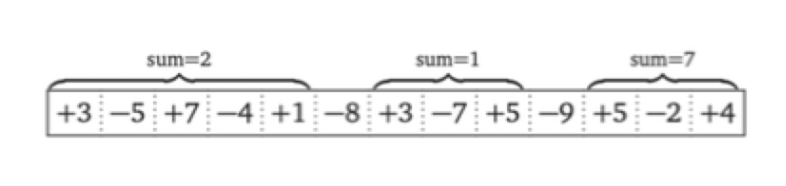
\includegraphics[width=0.65\textwidth]{positive-cover.png} \hspace{-0.15cm}
  \end{figure}

\end{problem}

\begin{solution}

  %=================================================
  % 1. THE ALGORITHM %=====================================================

  %=================================================
  % 2. PROOF OF CORRECTNESS %=====================================================

  %=================================================
  % 3. RUN TIME ANALYSIS %=====================================================

\end{solution}

\newpage

\begin{problem}
  We define a number to be \textbf{special} if it can be written as:
  \[
    n = a \cdot 197 + b \cdot 232
  \]
  where \(a\) and \(b\) are non-negative integers. For example:
  \begin{itemize}
    \item \(696\) is special because it can be written as \(696 = 0 \cdot 197 + 3 \cdot 232\).
    \item \(2412\) is special because it can be written as \(2412 = 4 \cdot 197 + 7 \cdot 232\).
    \item \(267\) is not special (since it cannot be written as \(a \cdot 197 + b \cdot 232\) for non-negative \(a\) and \(b\)).
  \end{itemize}

  The goal of this problem is to write a dynamic programming algorithm \textbf{Special(n)} that, given a positive integer \(n\), either finds non-negative integers \(a\) and \(b\) such that \(n = a \cdot 197 + b \cdot 232\), or returns “no solution” if no such \(a\) and \(b\) exist.

  Remember to separately write your specification of recursive formula in plain English , your recursive solution for the formula and its proof of correctness , the algorithm using either memoization or bottom-up dynamic programming , and runtime analysis.

\end{problem}

\begin{solution}

  %=================================================
  % 1. THE ALGORITHM %=====================================================

  %=================================================
  % 2. PROOF OF CORRECTNESS %=====================================================

  %=================================================
  % 3. RUN TIME ANALYSIS %=====================================================

\end{solution}

\newpage

\begin{problem}
  For the most part, we haven't been optimizing for space in our dynamic programs. But for many of the problems we've discussed it is possible to get away with much less space. The goal of this problem is for you do out one such example.

  Recall the subsetsum problem from class.
  INPUT: set $S=\left\{s_1, \ldots, s_n\right\}$ of non-negative integers and a target number $B$.
  OUTPUT: set $S^{\prime} \subseteq S$ with $\sum_{x \in S^{\prime}}=B$ or FALSE if no such $S^{\prime}$ exists.

  The algorithm we showed in class used $O(n B)$ time and $O(n B)$ space. Write pseudocode for an algorithm that solves subset sum in $O(n B)$ time but only needs $O(B)$ space in addition to the input itself. Your algorithm must return the actual set $S^{\prime}$.
\end{problem}

\begin{solution}

  %=================================================
  % 1. THE ALGORITHM %=====================================================

  %=================================================
  % 2. PROOF OF CORRECTNESS %=====================================================

  %=================================================
  % 3. RUN TIME ANALYSIS %=====================================================

\end{solution}

\newpage

\begin{problem}
  \textbf{ImportExport(A,B)}

  \textbf{Input:} Two arrays \(A[0 \ldots n-1]\) and \(B[0 \ldots n-1]\), both of length \(n\), representing the prices of tulips in country A and country B at different times, respectively. All entries in both arrays are positive integers.

  \textbf{Output:} Return the maximum possible profit, defined as:
  \[
    \max _{j>i} \{ B[j] - A[i] \}
  \]
  or return 0 if all such \( B[j] - A[i] \) are negative. You only need to return the value of the maximum profit, not the actual indices \(i\) and \(j\).

  \textbf{Example:}

  Given the input:

  \[
    A = [40, 18, 20, 25, 12, 13, 19, 20, 5, 7, 3]
  \]
  \[
    B = [15, 50, 5, 30, 34, 19, 28, 33, 20, 20, 20]
  \]

  The maximum possible profit is achieved by buying tulips at time \(i = 4\) (when \(A[4] = 12\)) and selling them at time \(j = 7\) (when \(B[7] = 33\)), which gives a profit of:
  \[
    B[7] - A[4] = 33 - 12 = 21
  \]

  Therefore, the output is \(21\).

  \begin{itemize}
    \item Give a recursive $O(n)$-time algorithm for ImportExport(A,B).

    \item Give a $O(n)$-time dynamic programming algorithm for ImportExport(A,B).
  \end{itemize}
\end{problem}

\begin{solution}

  %=================================================
  % 1. THE ALGORITHM %=====================================================

  %=================================================
  % 2. PROOF OF CORRECTNESS %=====================================================

  %=================================================
  % 3. RUN TIME ANALYSIS %=====================================================

\end{solution}

\newpage

\finishline

\begin{challenge}
  You are given a string consisting of just the characters $'a'$, $'b'$, or $'c'$. The task is to sort the string in lexicographical order ($a < b < c$) by finding the minimum number of swaps needed to achieve this. Each swap can exchange two characters in the string.

\end{challenge}

\end{document}